\documentclass[a4paper,12pt]{scrartcl}
\usepackage{pslatex} % -- times instead of computer modern

\usepackage[colorlinks=true,linkcolor=black,citecolor=black]{hyperref}
\usepackage{booktabs}
\usepackage{graphicx}

\usepackage[latin1]{inputenc}

\newcommand{\code}[1]{{\textsf{#1}}}
\newcommand{\sign}[1]{{\texttt{#1}}}


\begin{document}

\title{SimpCon -- a Simple SoC Interconnect\\Draft}
\author{Martin Schoeberl\\ martin@jopdesign.com}
\maketitle \thispagestyle{empty}

\begin{abstract}

This document proposes a simple interconnection standard for
system-on-chip (SoC) components. It is intended to provide pipelined
access to devices such on-chip peripherals and on-chip memory
controller with minimum hardware resources.


\end{abstract}

\section{Introduction}

The intention of the following SoC interconnect standard is to be
simple and efficient with respect to implementation resources and
transaction latency.

SimpCon is a fully synchronous standard for on-chip
interconnections. It is a point-to-point connection between a master
and a slave. The master starts either a read or write transaction.
Master commands are single cycle to free the master to continue on
internal operations during an outstanding transaction. The slave has
to register the address when needed for more than one cycle. The
slave also registers the data on a read and provides it to the
master for more than a single cycle. This property allows the master
to delay the actual read if it is busy with internal operations.

The slave signals the end of the transaction through a novel
\emph{ready counter} to provide an early notification. This early
notification simplifies the integration of peripherals into
pipelined masters.

Slaves can also provide several levels of pipelining. This feature
is announced by two static output ports (one for read and one write
pipeline levels).

Off-chip connections (e.g.\ main memory) are device specific and
need a slave to perform the translation. Peripheral interrupts are
not covered by this specification.

\subsection{Feature}

\begin{itemize}
    \item Master/slave point-to-point connection
    \item Synchronous operation
    \item Read and write transactions
    \item Early pipeline release for the master
    \item Pipelined transactions
    \item Open-source specification
    \item Low implementation overheads
\end{itemize}

\subsection{Basic Read Transaction}

Figure~\ref{fig:sc:basic:rd} shows a basic read transaction for a
slave with one cycle latency. The acknowledge signals are omitted
from the figure. In the first cycle, the address phase, the
\sign{rd} signals the slave to start the read transaction. The
address is registered by the slave. During the following cycle, the
read phase, the slave performs the read and registers the data. Due
to the register in the slave the data is available in the third
cycle, the result phase. To simplify the master, the read data stays
valid till the next read request response.

\begin{figure}
    \centering
    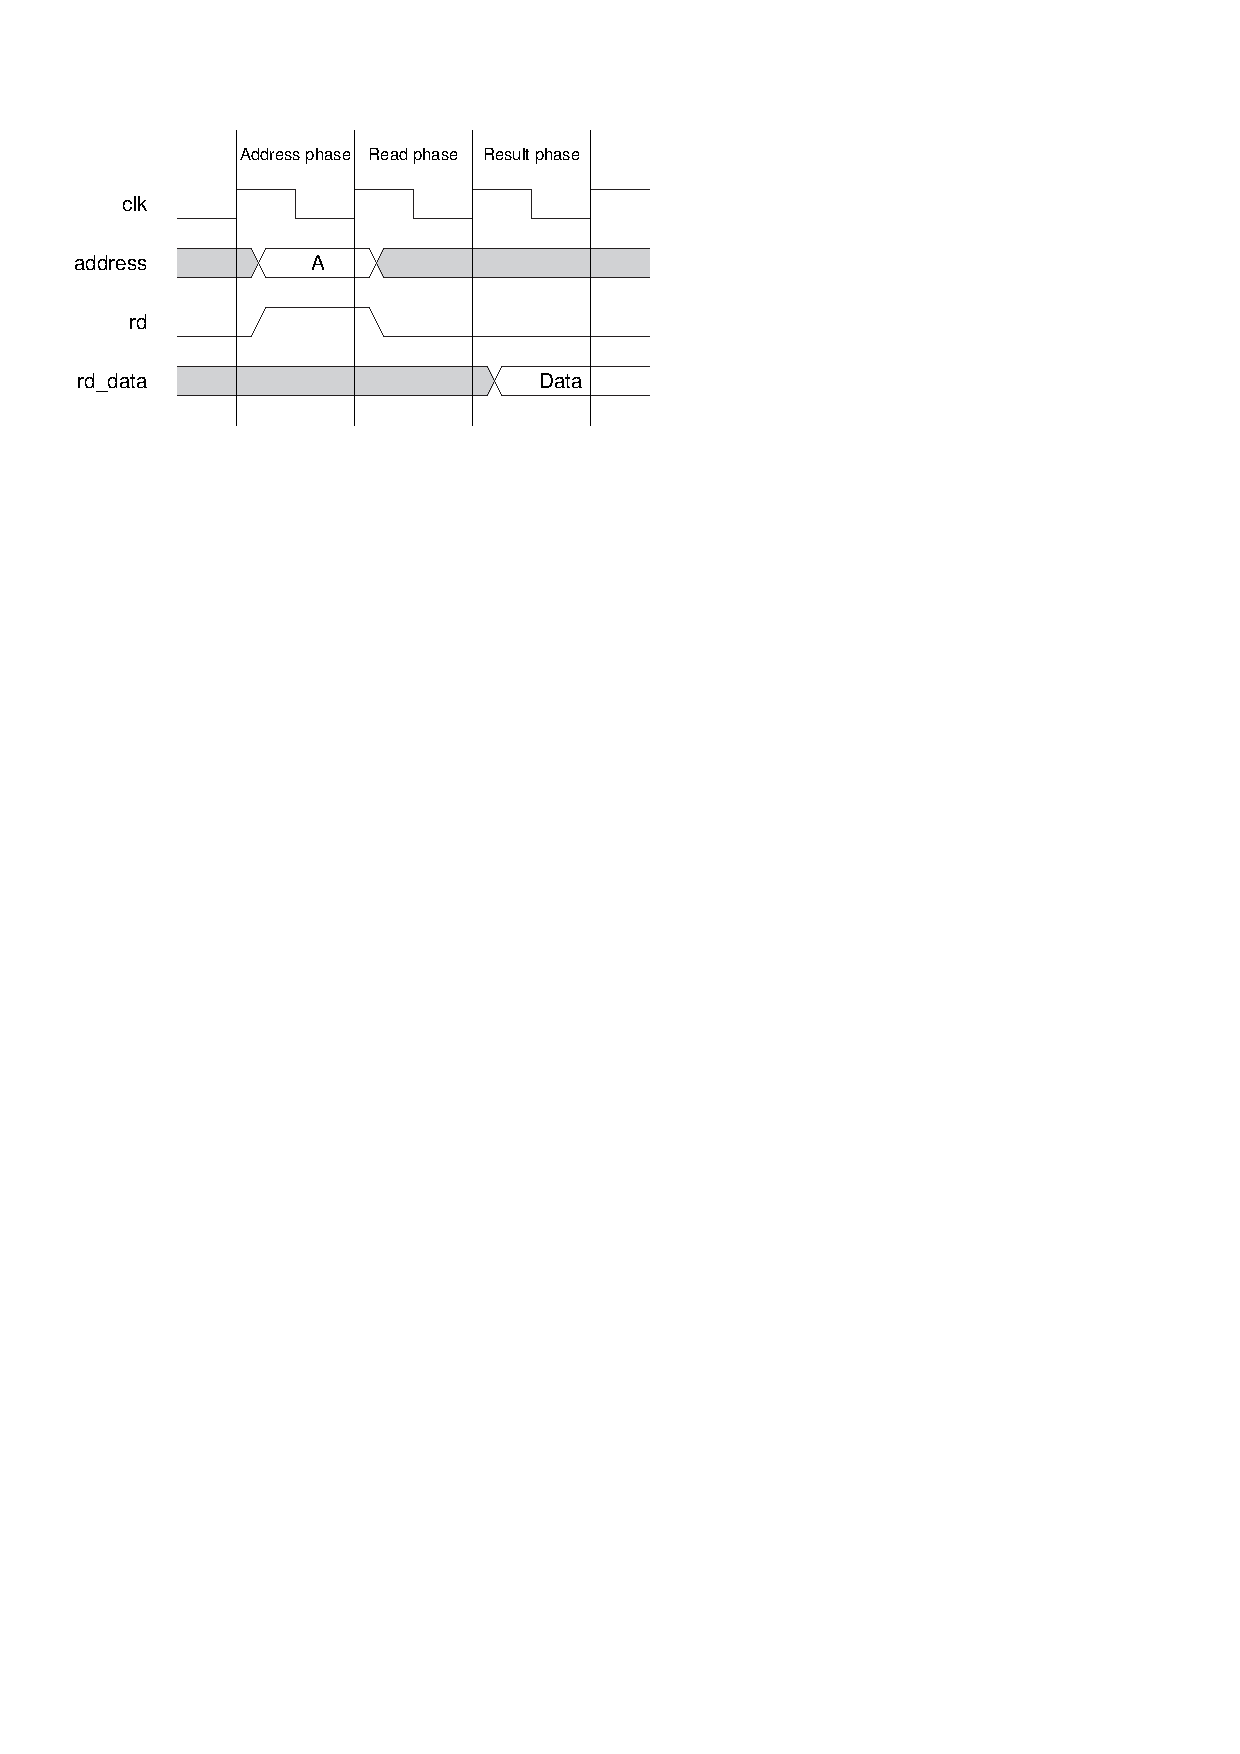
\includegraphics{figures/sc_basic_rd}
    \caption{Basic read transaction}
    \label{fig:sc:basic:rd}
\end{figure}

\subsection{Basic Write Transaction}

A write transaction consists of a single cycle address/command phase
started by assertion of \sign{wr} where the address and the write
data are valid. \sign{address} and \sign{wr\_data} are usually
registered by the slave. The end of the write cycle is signalled to
the master by the slave with \sign{rdy\_cnt}. See section
\ref{sec:ack} and an example in Figure~\ref{fig:sc:wr:ws}.

\section{SimpCon Signals}

This sections defines the signals used by the SimpCon connection.
Some of the signals are optional and may not be present on a
peripheral device.

All signals are a single direction point-to-point connection between
a master and a slave. The signal details are described by the device
that drives the signal. Table~\ref{tab:sc:signals} lists the signals
that define the SimpCon interface. The column Direction indicates
wether the signal is driven by the master or the slave.

\begin{table}
    \centering

    \begin{tabular}{lrlll}
        \toprule
        Signal & Width & Direction & Required & Description \\
        \midrule
        \sign{address} & 1--32 & Master & No & Address lines from the
        master\\
        & & & & to the slave port\\
        \sign{wr\_data} & 32 & Master & No & Data lines from the
        master\\
        & & & & to the slave port\\
        \sign{rd} & 1 & Master & No & Start of a read transaction \\
        \sign{wr} & 1 & Master & No & Start of a write transaction \\
        \sign{rd\_data} & 32 & Slave & No & Data lines from the
        slave\\
        & & & & to the master port\\
        \sign{rdy\_cnt} & 2 & Slave & Yes & Transaction end signalling \\
        \sign{rd\_pipeline\_level} & 2 & Slave & No & Maximum pipeline
        level\\
        & & & & for read transactions \\
        \sign{wr\_pipeline\_level} & 2 & Slave & No & Maximum pipeline
        level\\
        & & & & for write transactions \\
        \bottomrule

    \end{tabular}
    \caption{SimpCon port signals}
    \label{tab:sc:signals}

\end{table}



\subsection{Master Signal Details}

This section describes the signals that are driven by the master to
initiate a transaction.

\subsubsection{address}

Master addresses represent word addresses as offsets in the slaves
address range. \sign{address} is valid a single cycle either with
\sign{rd} for a read transaction or with \sign{wr} and
\sign{wr\_data} for a write transaction.

The number of bits for \sign{address} depend on the slaves address
range. For a single port slave \sign{address} can be omitted.

\subsubsection{wr\_data}

The \sign{wr\_data} signals carry the data for a write transaction.
It is valid for a single cycle together with \sign{address} and
\sign{wr}. The signal is typically 32 bits wide. Slaves can ignore
upper bits when the slave port is less than 32 bits.

\subsubsection{rd}

The \sign{rd} signal is asserted a single clock cycle to start a
read transaction. \sign{address} has to be valid in the same cycle.

\subsubsection{wr}

The \sign{wr} signal is asserted a single clock cycle to start a
write transaction. \sign{address} and \sign{wr\_data} have to be
valid in the same cycle.

\subsubsection{sel\_byte}

The \sign{sel\_byte} signal is reserved for future versions of the
SimpCon specification to add individual byte enables.

\subsection{Slave Signal Details}

This section describes the signals that are driven by the slave as a
response to transaction initiated by the master.

\subsubsection{rd\_data}

The \sign{wr\_data} signals carry the result for a read transaction.
The data is valid when \sign{rdy\_cnt} reaches 0 and stays valid
till a new read result is available. The signal is typically 32 bits
wide. Slaves that provide less than 32 bits should pad the upper
bits with 0.

\subsubsection{rdy\_cnt}

The \sign{rdy\_cnt} signal provides the number of cycles till the
pending transaction will finish. A 0 means that either read data is
available or a write transaction has been finished. Values of 1 and
2 mean the the transaction will finish in at least 1 or 2 cycles.
The maximum value is 3 and means the the transaction will finish in
3 or \emph{more} cycles. Note that not all values have to be used in
a transaction. Each monotonic sequence of \sign{rdy\_cnt} values is
legal.

\subsubsection{rd\_pipeline\_level}

The static \sign{rd\_pipeline\_level} provides the master with the
read pipeline level of the slave. The signal has to be constant to
enable the synthesizer to optimize the pipeline level dependent
state machine in the master.


\subsubsection{wr\_pipeline\_level}

The static \sign{wr\_pipeline\_level} provides the master with the
write pipeline level of the slave. The signal has to be constant to
enable the synthesizer to optimize the pipeline level dependent
state machine in the master.

\section{Slave Acknowledge}
\label{sec:ack}

Flow control between the slave and the master is usually done by a
single signal in the form of \emph{wait} or \emph{acknowledge}. The
\sign{ack} signal, e.g.\ in the Wishbone specification, is set when
the data is available or the write operation has finished. However,
for a pipelined master it can be of interest to know it
\emph{earlier} when a transaction will finish.

For a lot of slaves, e.g.\ a SRAM interface with fixed wait states,
this information is available inside the slave. In the SimpCon
interface this information is communicated to the master through the
two bit signal \sign{rdy\_cnt}. \sign{rdy\_cnt} signals the number
of cycles till the read data will be available or the write
transaction will be finished. Value 0 is equivalent to an \emph{ack}
signal and 1, 2, and 3 are equivalent to a wait request with the
distinction that the master knows how long the wait request will
last.

To avoid too many signals at the interconnect \sign{rdy\_cnt} has a
width of two bits. Therefore, the maximum value of 3 has the special
meaning that the transaction will finish in 3 or \emph{more} cycles.
As a result the master can only use the values 0, 1, and 2 to
release actions in it's pipeline.

Idle slaves will keep the former value of 0 for \sign{rdy\_cnt}.
Slaves, that don't know in advance how many wait states are need for
the transaction can produce sequences that omit any of the numbers
3, 2, and 1. The master has to handle this situations.

Figure~\ref{fig:sc:rd:ws} shows an example of a slave that needs
three cycles for the read to be processed. In cycle 1 the read
command and the address are set by the master. The slave registers
the address and sets \sign{rdy\_cnt} to 3 in cycle 2. The read takes
three cycles (2--4) during which \sign{rdy\_cnt} is decremented. In
cycle 4 the data is available inside the slave and gets registered.
It is available in cycle 5 for the master and \sign{rdy\_cnt} is
finally 0. Both, the \sign{rd\_data} and \sign{rdy\_cnt} will keep
their value till a new transaction is requested.

\begin{figure}
    \centering
    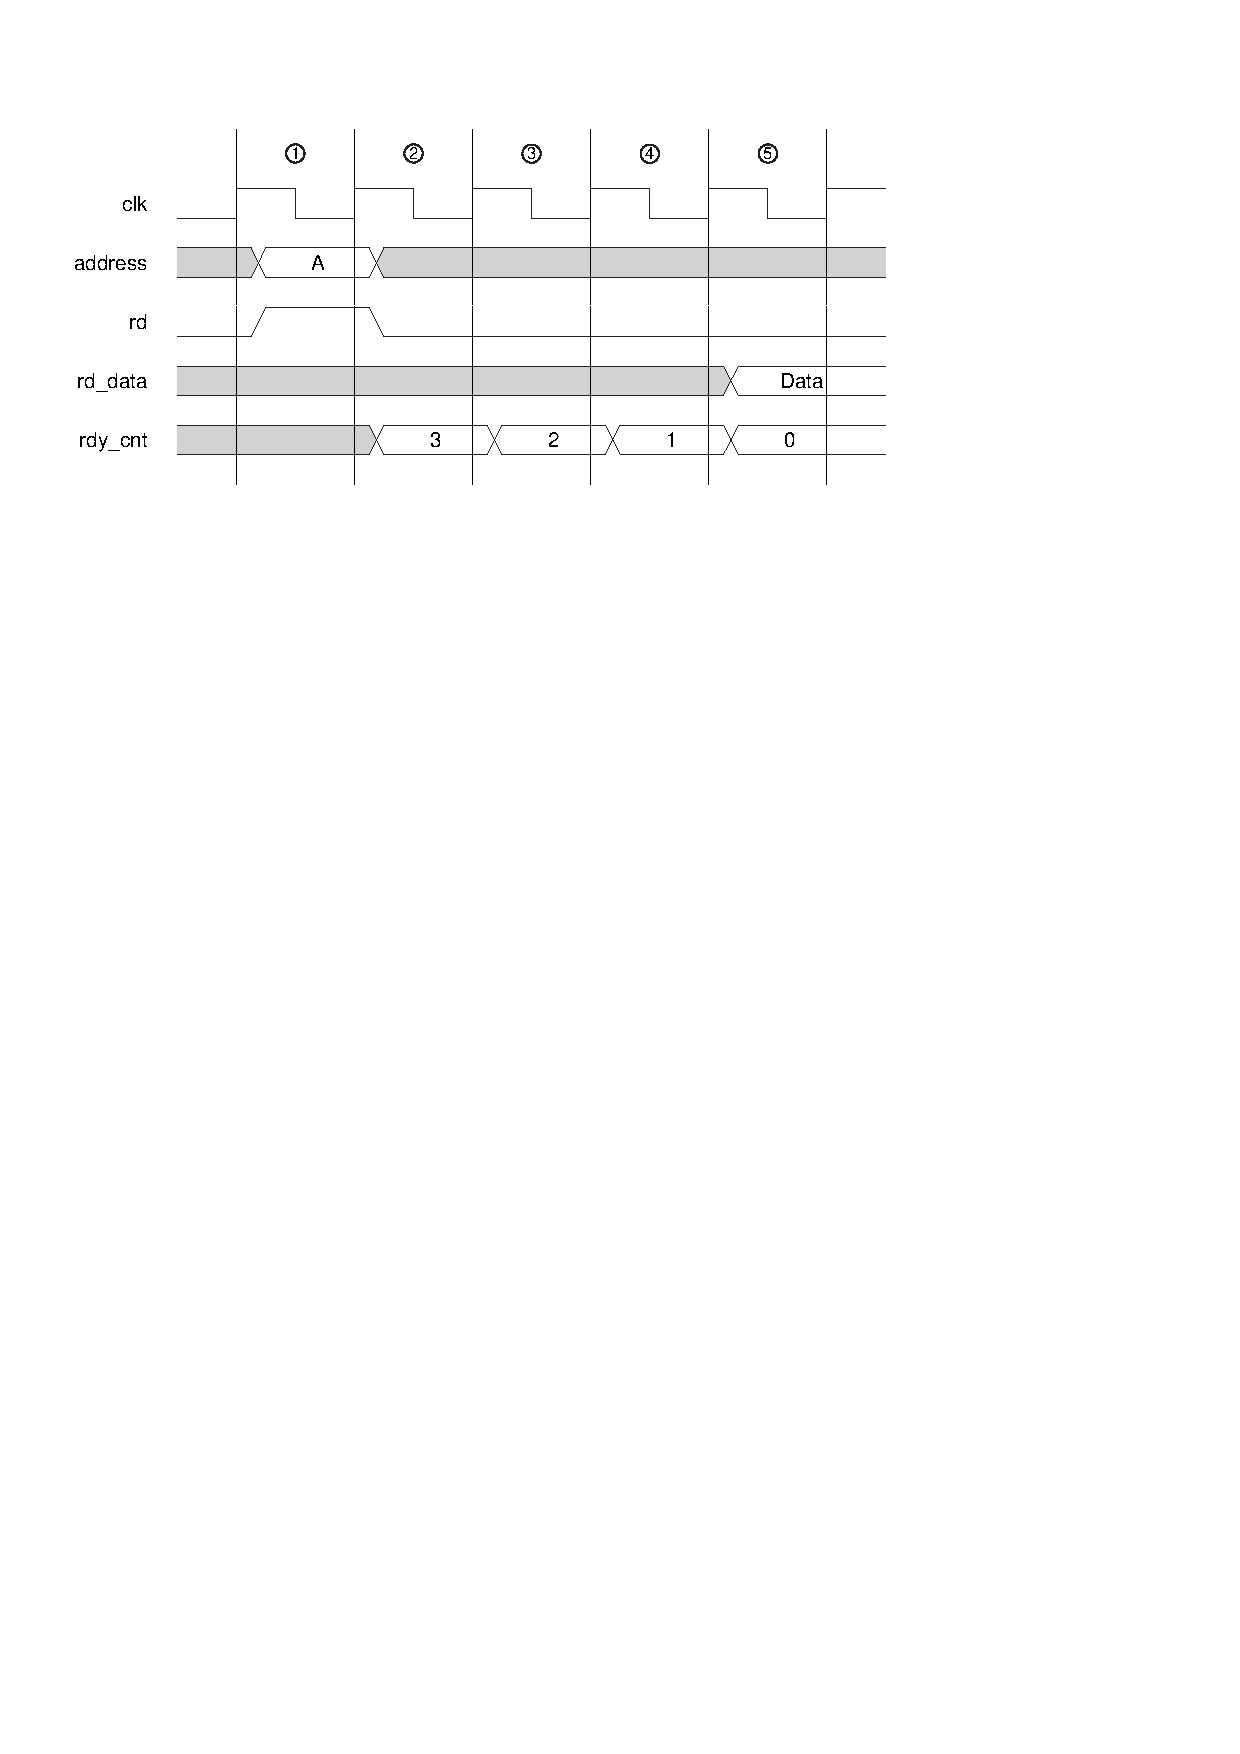
\includegraphics{figures/sc_rd_ws}
    \caption{Read transaction with wait states}
    \label{fig:sc:rd:ws}
\end{figure}


Figure~\ref{fig:sc:wr:ws} shows an example of a slave that needs
three cycles for the write to be processed. The address, the data to
be written and the write command are valid during cycle 1. The slave
registers the address and write data during cycle 1 and performs the
write operation during cycles 2--4. The \sign{rdy\_cnt} is
decremented and a non-pipelined slave can accept a new command after
cycle 4.

\begin{figure}
    \centering
    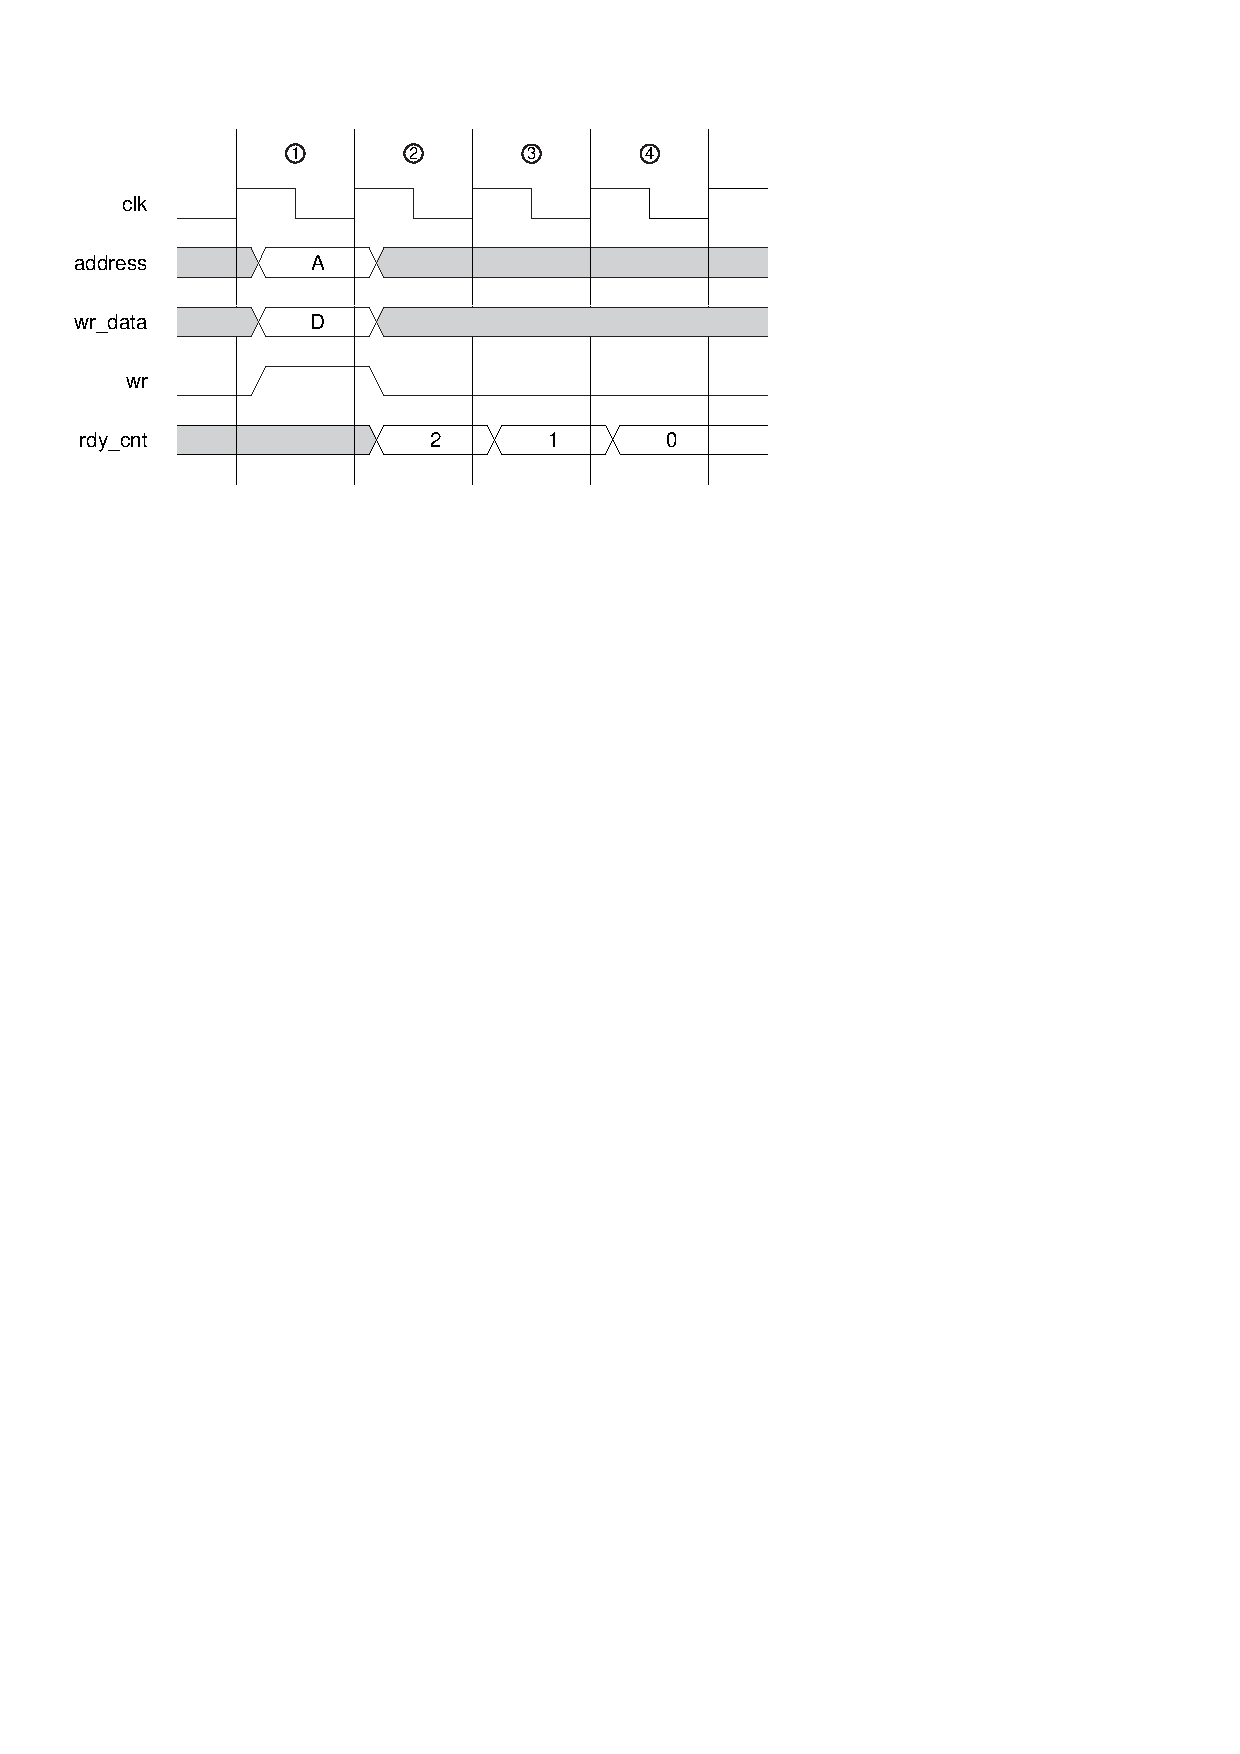
\includegraphics{figures/sc_wr_ws}
    \caption{Write transaction with wait states}
    \label{fig:sc:wr:ws}
\end{figure}



\section{Pipelining}

Figure~\ref{fig:sc:pipe:level} shows a read transaction for a slave
with four cycles latency. Without any pipelining the next read
transaction will start in cycle 7 after the data from the former
read transaction is read by the master. The three bottom lines show
when new read transactions will be started for different pipeline
levels. With pipeline level 1 a new transaction can start in the
same cycle when the former read data is available (in this example
in cycle 6). Higher levels mean that the next read will start
earlier as shown for level 2 and 3.

\begin{figure}
    \centering
    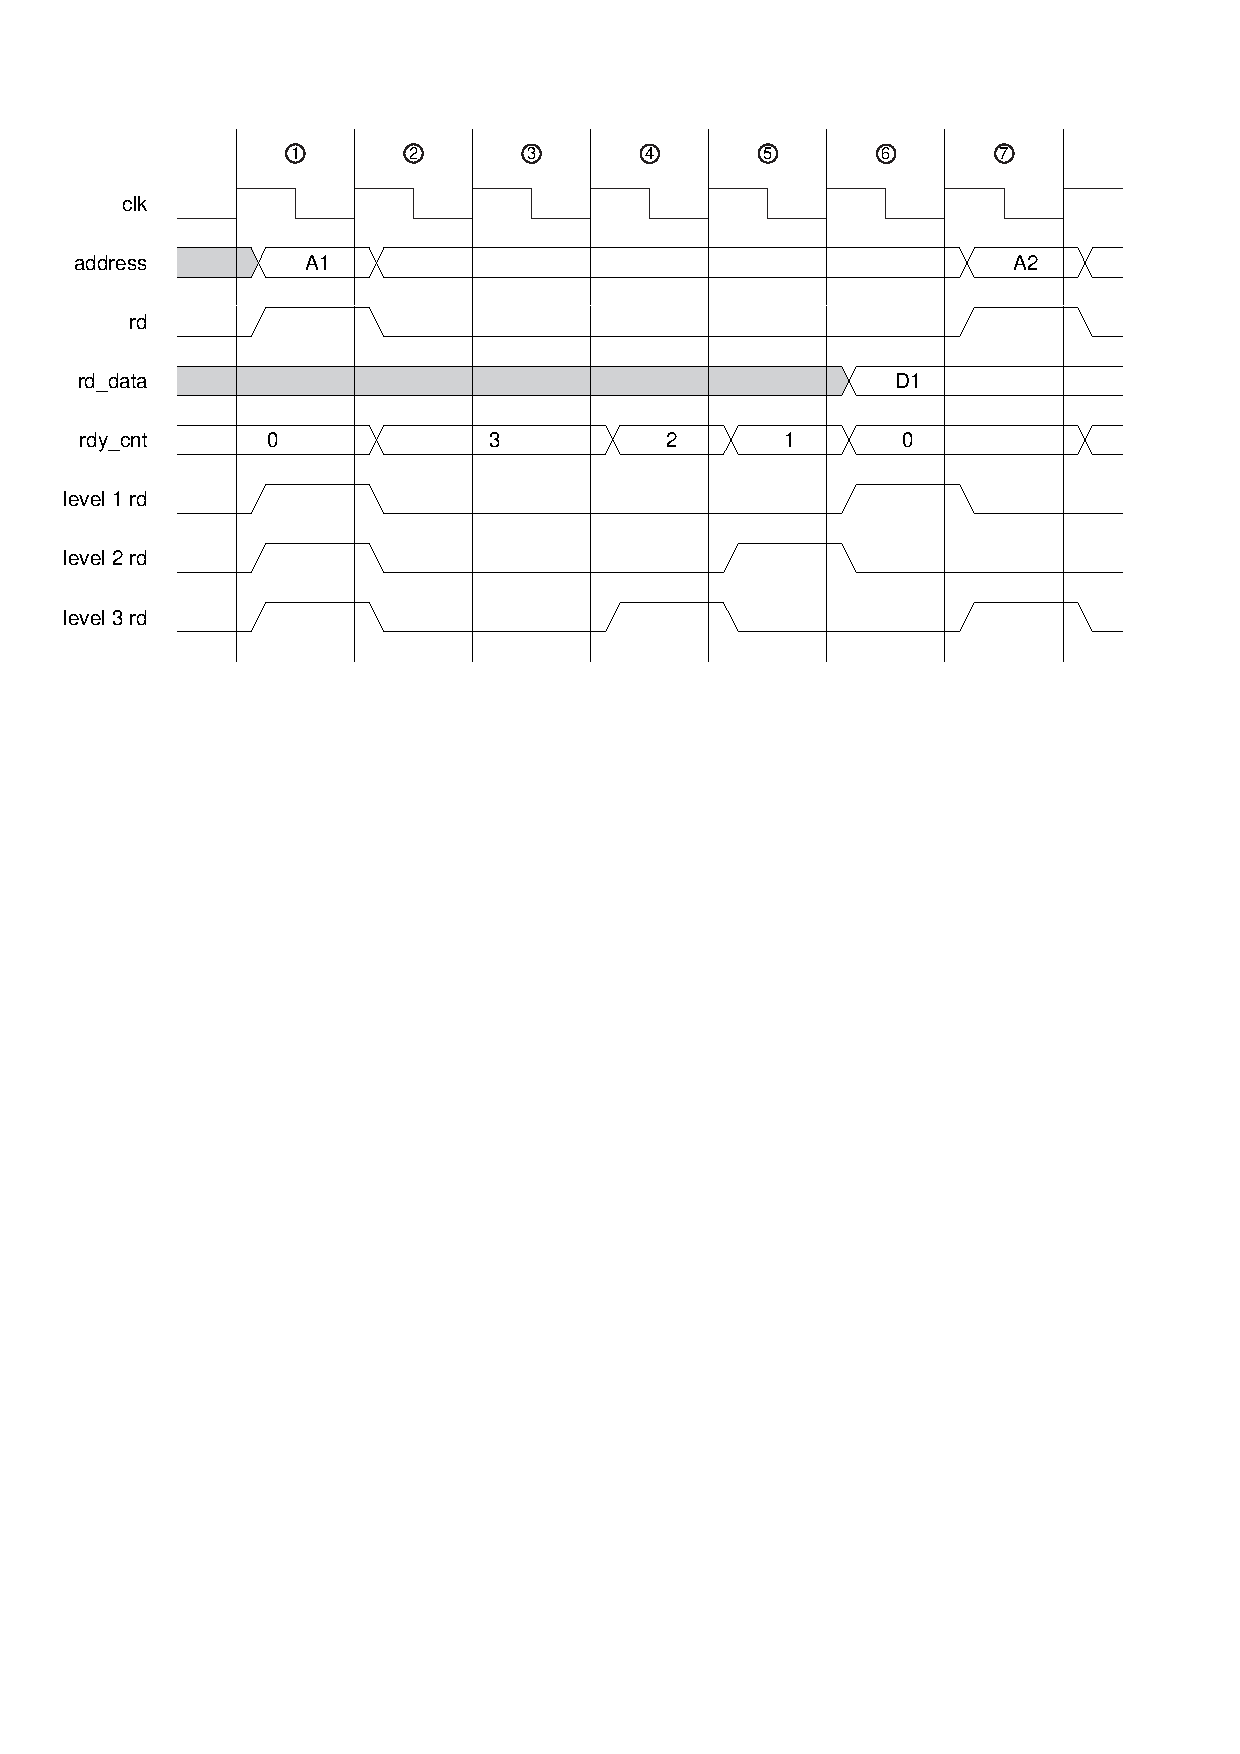
\includegraphics[width=\textwidth]{figures/sc_pipe_level}
    \caption{Different pipeline levels for a read transaction}
    \label{fig:sc:pipe:level}
\end{figure}

Implementation of level 1 in the slave is trivial (just two more
transitions in the state machine). It is recommended to provide
level 1 at least for read transactions. Level 2 is a little bit more
complex but usually no additional address or data registers are
needed.

To implement level 3 pipelining in the slave at least an additional
address register is needed. However, to use level 3 the master has
to issue the request in the same cycle as \sign{rdy\_cnt} goes to 2.
That means this transition is combinatorial. We see in
Figure~\ref{fig:sc:pipe:level} that \sign{rdy\_cnt} value of 3 means
three or more cycles till the data is available and can therefore
not be used to trigger a new transaction.

\section{Multiple Master}

SimpCon defines no signals for the communication between a master
and an arbiter. However, it is possible to build a multi master
system with SimpCon. The SimpCon interface can be used as
interconnect between the masters and the arbiter and the arbiter and
the slaves. In this case the arbiter acts as slave for the master
and as master for the peripheral devices.

The missing arbitration protocol in SimpCon results in the need to
queue $n-1$ requests in an arbiter for $n$ masters. However, for
this additional HW we get zero overheads for the bus request. The
master, which gets the bus will will start the slave transaction in
the same cycle.
\\
\\
TODO: add a timing diagram to explain this concept.


\section{Examples}

This section provides some examples for the application of the
SimpCon definition.

\subsection{IO Port}

TODO: Show how simple an IO port can be with SimpCon. We need no
addresses and can tie \sign{bsy\_cnt} to 0. We only need the
\sign{rd} or \sign{wr} signal to enable the port.

\subsection{SRAM interface}

The following example is taken from an implementation of SimpCon for
a Java processor. The processor is clocked with 100MHz and the main
memory consists of 15ns static RAMs. Therefore the minimum access
time for the RAM is two cycles. The slack time of 5ns forces us to
use output registers for the RAM address and write data and input
registers for the read data in the IO cells of the FPGA. These
registers fit nice with the intention of SimpCon to use registers
inside the slave.

Figure~\ref{fig:sc:sram} shows the interface for a non-pipelined
read access followed by a write access. Four signals are driven by
the master and two signal by the slave. The lower half of the figure
shows the signals at the FPGA pins where the RAM is connected.

\begin{figure}
    \centering
    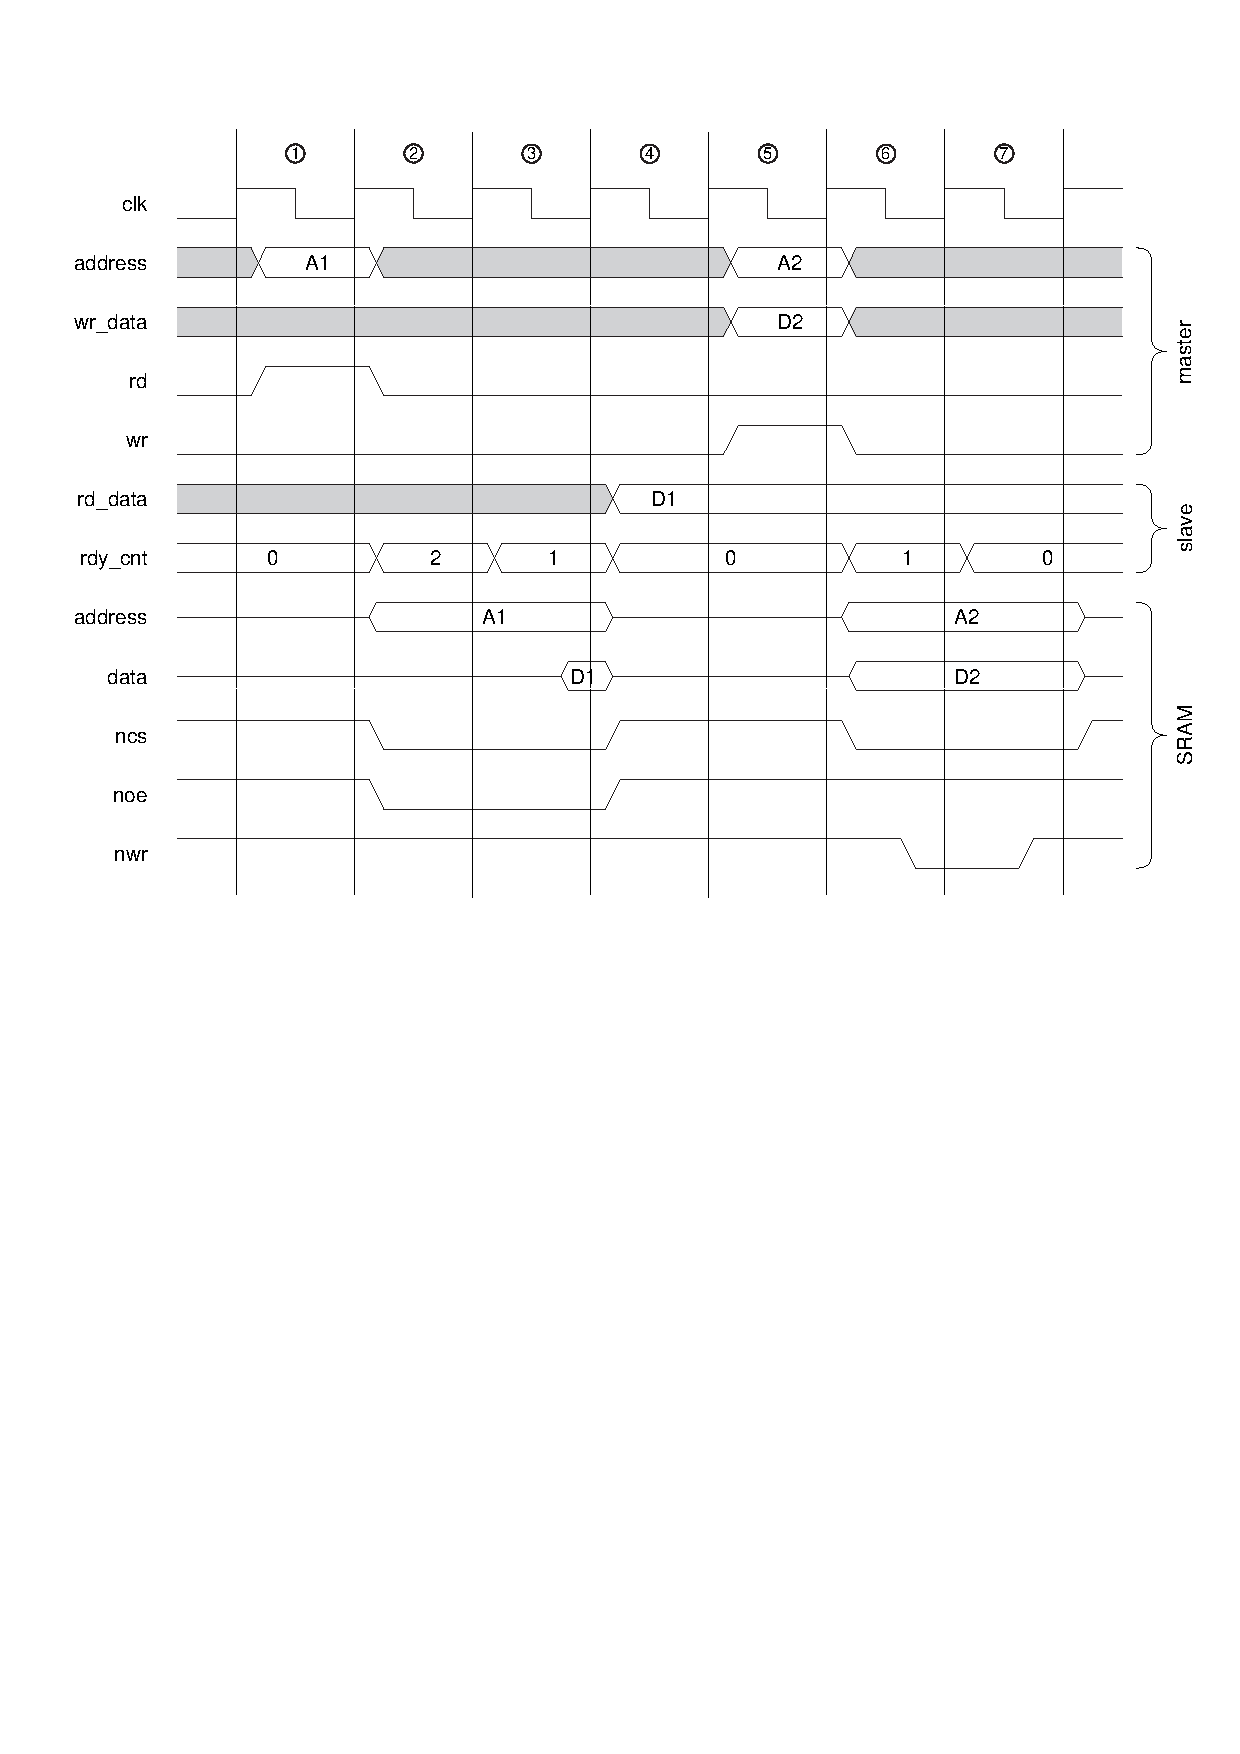
\includegraphics[width=\textwidth]{figures/sc_sram}
    \caption{Static RAM interface without pipelining}
    \label{fig:sc:sram}
\end{figure}

In cycle 1 the read transaction is started by the master and the
slave registers the address. The slave also sets the registered
control signals \sign{ncs} and \sign{noe} during cycle1. Due to the
IO cell registers, the address and control signals are valid at the
FPGA pins very early in cycle 2. At the end of cycle 3 (15ns after
\sign{address}, \sign{ncs} and \sign{noe} are stable) the data from
the RAM is available and can be sampled with the rising edge for
cycle 4.

The master reads the data in cycle 4 and starts a write transaction
in cycle 5. Address and data are again registered from the slave and
are available for the RAM at the beginning of cycle 6. To perform a
write in two cycles the nwr signal is registered by a negative
triggered flip-flop.

In figure~\ref{fig:sc:sram:prd} we see a pipelined read from the RAM
with pipeline level 2. With this pipeline level and the two cycles
read access time of the RAM we get the maximum bandwidth possible.

\begin{figure}
    \centering
    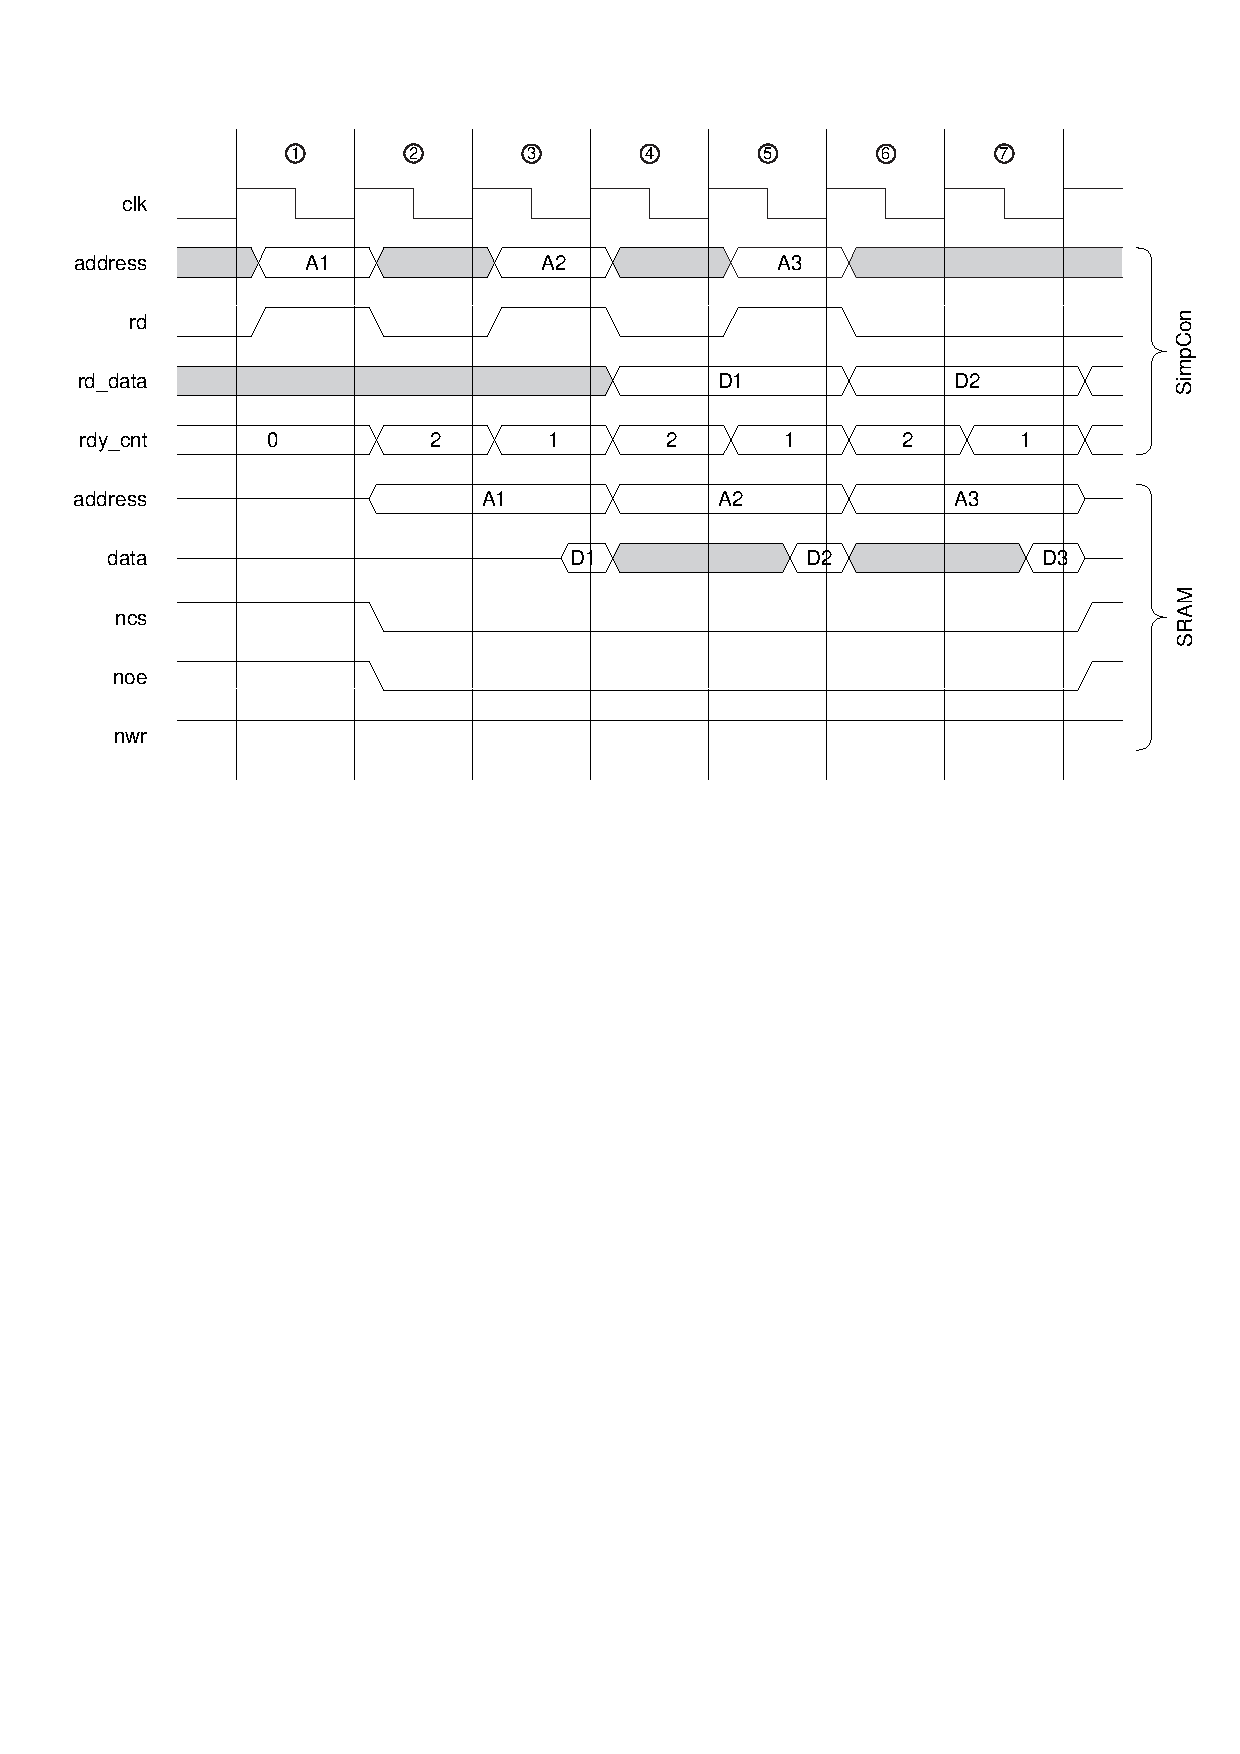
\includegraphics[width=\textwidth]{figures/sc_sram_prd}
    \caption{Pipelined read from a static RAM}
    \label{fig:sc:sram:prd}
\end{figure}

We can see the start of the second read transaction in cycle 3
during the read of the first data from the RAM. The new address is
registered in the same cycle and available for the RAM in the
following cycle 4. Although we have a pipeline level of 2 we need no
additional address or data register. The read data is available for
two cycles (\sign{rdy\_cnt} 2 or 1 for the next read) and the master
is free to select one of the two cycles to read the data.

\subsection{Master Multiplexing}

To add several slaves to a single master the \sign{rd\_data} and
\sign{bsy\_cnt} have to be multiplexed. Due to the fact that all
\sign{rd\_data} signals are registered by the slaves a single
pipeline stage will be enough for a large multiplexer. The selection
of the multiplexer is also known at the transaction start but needed
at most in the next cycle. Therefore it can be registered to further
speed up the multiplexer.
\\
\\
TODO: add a schematic for the master \sign{rd\_data} multiplexer.

\section{Status}

\begin{itemize}
    \item First timing diagrams drawn
    \item SimpCon SRAM interface for JOP on Cyclone and Spartan-3 is
    available
    \item Project at opencores.org accepted
\end{itemize}
%
Next steps:
%
\begin{itemize}
    \item Continue this document
    \item Provide more SimpCon examples (e.g.\ a UART)
    \item Change JOPs IO interface to SimpCon
    \item Provide Wishbone bridges
\end{itemize}
%
to clarify:
\begin{itemize}
    \item Use transaction or transfer in this document?
    \item Use address phase or better command cycle?
\end{itemize}

\end{document}


\section{Notes}

\subsection{Group comment}

After implementing the Wishbone interface for main memory access
from JOP I see several issues with the Wishbone specification that
makes it not the best choice for SoC interconnect.

The Wishbone interface specification is still in the tradition of
microcomputer or backplane busses. However, for a SoC interconnect,
which is usually point-to-point, this is not the best approach.

The master is requested to hold the address and data valid through
the whole read or write cycle. This complicates the connection to a
master that has the data valid only for one cycle. In this case the
address and data have to be registered \emph{before} the Wishbone
connect or an expensive (time and resources) MUX has to be used. A
register results in one additional cycle latency. A better approach
would be to register the address and data in the slave. Than there
is also time to perform address decoding in the slave (before the
address register).

There is a similar issue for the output data from the slave: As it
is only valid for a single cycle it has to be registered by the
master when the processor is not reading it immediately. Therefore,
the slave should keep the last valid data at it's output even when
\emph{wb.stb} is not assigned anymore (which is no issue from the
hardware complexity).

The Wishbone connection for JOP resulted in an unregistered Wishbone
memory interface and registers for the address and data in the
Wishbone master. However, for fast address and control output
($t_{co}$) and short setup time ($t_{su}$) we want to place the
registers in the IO-pads of the FPGA. With the registers are buried
in the WB master it takes some effort to set the right constraints
for the Synthesizer to implement such IO-registers.

The same issue is true for the control signals. The translation from
the \emph{wb.cyc}, \emph{wb.stb} and \emph{wb.we} signals to
\emph{ncs}, \emph{noe} and \emph{nwe} for the SRAM are on the
critical path.

The \emph{ack} signal is too late for a pipelined master. We would
need to know it *earlier* when the next data will be available ---
and this is possible, as we know in the slave when the data from the
SRAM will arrive. A work around solution is a non-WB-conforming
early ack signal.

Due to the fact that the data registers not inside the WB interface
we need an extra WB interface for the Flash/NAND interface (on the
Cyclone board). We cannot afford the address decoding and a MUX in
the data read path without registers. This would result in an extra
cycle for the memory read due to the combinational delay.

In the WB specification (AFAIK) there is no way to perform pipelined
read or write. However, for blocked memory transfers (e.g. cache
load) this is the usual way to get a good performance.

Conclusion -- I would prefer:

    * Address and data (in/out) register in the slave
    * A way to know earlier when data will be available (or
      a write has finished)
    * Pipelining in the slave

As a result from this experience I'm working on a new SoC
interconnect (working name SimpCon) definition that should avoid the
mentioned issues and should be still easy to implement the master
and slave.

As there are so many projects available that implement the WB
interface I will provide bridges between SimpCon and WB. For IO
devices the former arguments do not apply to that extent as the
pressure for low latency access and pipelining is not high.
Therefore, a bridge to WB IO devices can be a practical solution for
design reuse.

\subsubsection{additional comments}

The idea for (some) pipeline support is twofold:

1.) The slave will provide more information than a single \emph{ack}
or wait states. It will (if it is capable to do) signal the number
of clock cycles remaining till the read data is available (or the
write has finished) to the master. This feature allows the pipelined
master to prepare for the upcoming read.

2.) If the slave can provide pipelining the master can use
overlapped wr or rd requests. The slave has a static output port
that tells how many pipeline stages are available. I call this
'pipeline level':
    0 means non overlapping
    1 a new rd/wr request can be issued in the same cycle
      when the former data is read.
    2 one earlier and
    3 is the maximum level where you get full pipelining
      on the basic read cycle with one wait state
      (command - read - read - result).


The draft of the spec at the moment are few sketches on real paper -
takes some time to draw all diagrams for a document.

I have a first implementation of SimpCon on JOP to test the ideas: A
master in JOP and a slave for SRAM access.
